\documentclass{article}
\usepackage{graphicx}
\usepackage{hyperref}
\usepackage{amsmath}

% Title content
\title{Transferability of Adversarial Reinforcement Learning}
\author{Connor Fuhrman, Johnathan Gill}
\date{May 11 2021}

\begin{document}

\maketitle

\begin{abstract}
It is well known that deep learning and deep reinforcement learning (RL) are vulnerable to adversarial attacks via a model's observations. 
Recently, it was shown that RL is susceptible to adversarial attacks on the \textit{policy} alone via an attacker trained to develop an adversarial policy. 
Such attacks are especially interesting because the adversarial attacker does not simply perturb the victim's model's input, i.e., in RL the observation space, but rather choses physically realistic actions such that the victim's policy breaks down. 
This method of adversarial attack is especially interesting because real-world RL agents may only interact with each other and the environment around them in a physically realistic fashion. 
This work investigates the transferability of such adversarial policies between various model architectures via a "shoot and defend" type game. 
Quadcopter agents are trained to be either the shooter, who's goal is to shoot a ball into a goal, or a defender, who's goal is to keep the ball out of the goal. 
There are two shooter agents trained with varying model architectures and two keeper agents, one of which is trained adversarially against one shooter agent but \texttt{not} the other. 
We find that ...
\end{abstract}

\newpage

\section{Introduction}\label{sec:intro}
Adversarial attacks against neural network classifiers and (deep) reinforcement learning (RL) has been shown effective via adversarial perturbations of the victim model's input, e.g., altering pixel values for an image classifier or perturbing an observation space for an RL model. 
However, such attacks are artificial when considering real-world RL agents as an adversarial attacker cannot directly alter image pixel or observation space values but can only interact naturally with the environment and the victim model, e.g., an adversarial attack against an autonomous unmanned aerial vehicle (UAV) cannot access the UAV's perception equipment directly to alter measurement values nor can it alter the environment in a non-physically realistic manner. 
\\ \\ 
\noindent 
Work done in \cite{Gleave2019} showed that an adversarial policy was effective in multiple zero-sum games, including shoot and defend where the \textit{shooter} agent attempts to shoot a ball into a goal while the \textit{keeper} agent seeks to keep the ball out of the goal. 
The adversarial attacker, the keeper agent, demonstrated significantly different activations than the normal models and was overall successful in each game by manipulating only it's own body position to exploit weaknesses in the victim's (the shooter agent) policy.
Videos showing the results from \cite{Gleave2019} are available \href{https://adversarialpolicies.github.io/}{online} and show that adversarial policies are more effective in higher-dimensional spaces such as humanoid models over lower-dimensional spaces such as ants. 

\begin{figure}[h!]
  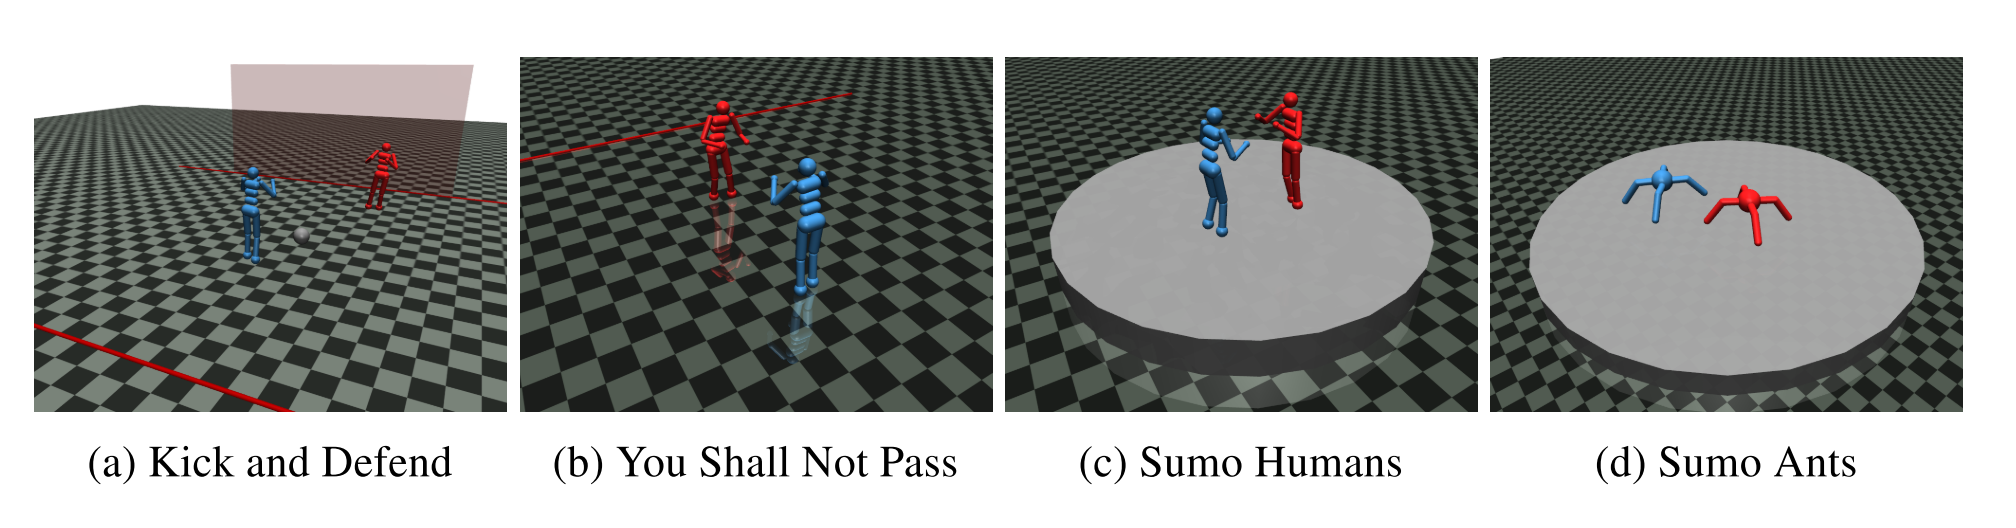
\includegraphics[width=\linewidth]{imgs/Gleave2019_env}
  \caption{Training environment used in \cite{Gleave2019} showing all four zero-sum games investigated for adversarial policies}
  \label{fig:gleave_env}
\end{figure}

\noindent 
The adversarial agents in \cite{Gleave2019} were given unlimited black-box access to the victim's policy, $\pi_v$, but were not given any white-box access to model weights or activations. 
The victim model's policy was frozen and actions were sampled from the stochastic policy such that $a_v$ is a sample of the stochastic policy $\pi_v(. | s)$ while the adversary developed a policy $\pi_a$ such that $\pi_a$ maximizes the discounted sum of rewards. 
Agents trained adversarially demonstrate reliable domination of the vicim models, winning upwards of 90\% of games in most cases. 
However, it is interesting to note that when the victim is "blind" to the attacker, i.e., the victim's observations corresponding to the attacker's position is set statically to a typical initial value, its performance increases significantly from losing over 80\% of games to winning 99\% of games in \textit{You Shall Not Pass} (this game demonstrates the phenomenon best but the trend exists in other games). 

\section{Methods}\label{sec:methods}
The following sections discuss the gym environment, RL framework, and deployment on the high performance computing (HPC) cluster at the University of Arizona.

\subsection{Gym Environment}\label{subsec:gym_env}
We utilize an OpenAI-based gym environment introduced in \cite{Panerati2021} which provides a multi-agent RL environment based on the \texttt{Bullet} physics engine. 
The environment, \texttt{gym-pybullet-drones}, (original repository available online at \url{github.com/utiasDSL/gym-pybullet-drones}) allows users to rapidly create new environments and instantiate models within defined by their Unified Robot Description Format (URDF). \\ \\
\noindent
The drone model utilized in this work is the \href{https://www.bitcraze.io/documentation/hardware/crazyflie_2_1/crazyflie_2_1-datasheet.pdf}{Bitcraze Cracyflie 2.1} as this model ships with the gym environment. 
The quadcopter itself is a small open-source development platform which weight under 30g and is intended for education, research, and in particular swarm applications. 
Note, however, that these models in particular are not integral to this work but were chosen simply because they were readily available.

\subsection{Shoot and Defend Environment}
The \textit{Shoot and Defend} environment is configured as in Figure~\ref{fig:sad_env}. 
The shooter and defender agents are each constrained to remain in their respective areas and recivee a punishment if this boundary is violated. 
The shooter agent receives a reward if the ball enters the goal area and a penalty if the ball goes out of bounds or becomes stationary. 

\begin{figure}
  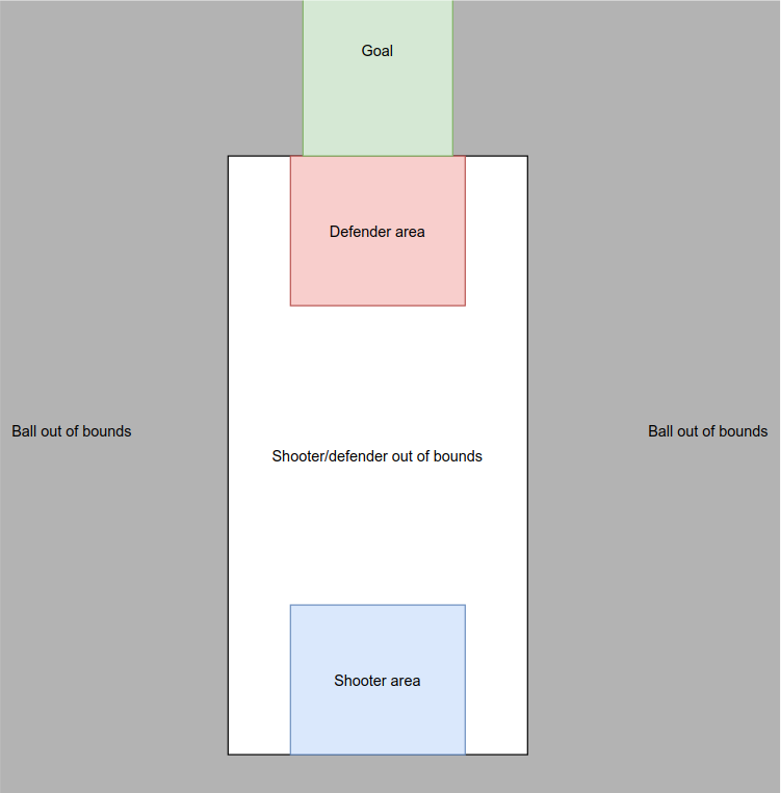
\includegraphics[width=\linewidth]{imgs/ShootAndDefend_env}
  \caption{Diagram depicting the \textit{Shoot and Defend} environment. Note this is a top-down view as the shooter and defender may travel in the vertical direction.}
  \label{fig:sad_env}
\end{figure}


\newpage
\bibliographystyle{plain}
\bibliography{reference.bib}

\end{document}